\subsubsection{Cenário Yaw}

Neste cenário, o objetivo é analisar o comportamento do controlador do quadricóptero ao ser submetido a uma mudança de guinada (yaw), enquanto os controladores dos outros eixos (pitch, roll e altitude) mantêm o quadricóptero estável em sua posição e altitude.

\begin{figure}[H]
    \centering
    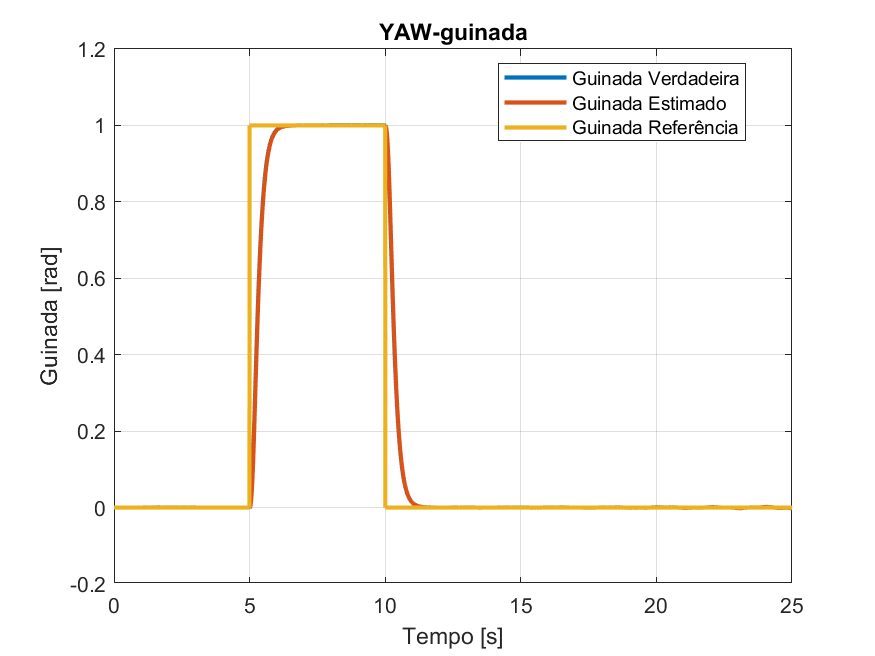
\includegraphics[width=0.8\textwidth]{YAW-guinada.png}
    \caption{Resposta do Yaw para o Cenário de Mudança de Yaw}
    \label{fig:YAW-guinada}
\end{figure}

No gráfico da guinada (Figura \ref{fig:YAW-guinada}), observamos que o sistema responde rapidamente à mudança no ângulo de yaw, acompanhando a referência quase instantaneamente, com uma resposta sem oscilação significativa após a estabilização. A curva estimada (linha laranja) acompanha bem a referência (linha amarela), indicando que o controlador de yaw está bem ajustado para esse tipo de movimento.

\begin{figure}[H]
    \centering
    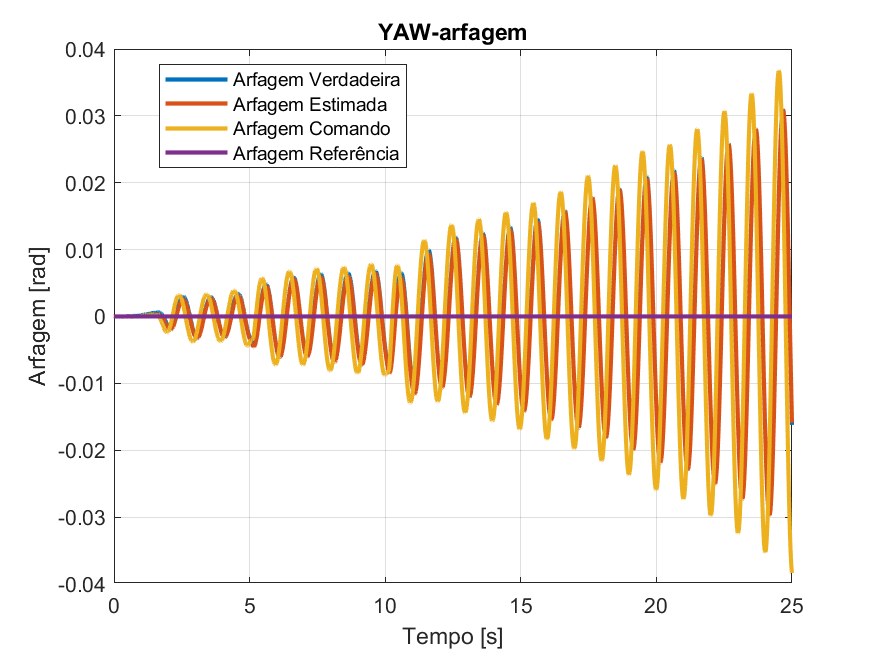
\includegraphics[width=0.8\textwidth]{YAW-arfagem.png}
    \caption{Resposta da Arfagem para o Cenário de Mudança de Yaw}
    \label{fig:YAW-arfagem}
\end{figure}

No gráfico da arfagem (Figura \ref{fig:YAW-arfagem}), é possível notar oscilações de pequena amplitude ao longo do tempo, mostrando uma leve oscilação residual como resposta à mudança de yaw. Essas oscilações indicam uma resposta cruzada mínima que não afeta significativamente a estabilidade geral do sistema.

\begin{figure}[H]
    \centering
    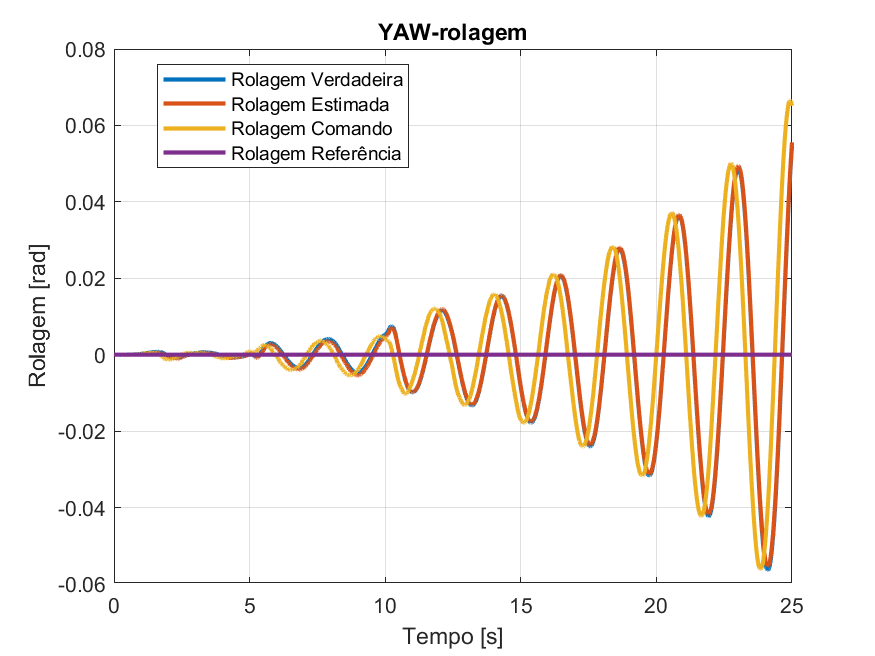
\includegraphics[width=0.8\textwidth]{YAW-rolagem.png}
    \caption{Resposta da Rolagem para o Cenário de Mudança de Yaw}
    \label{fig:YAW-rolagem}
\end{figure}

A resposta da rolagem (Figura \ref{fig:YAW-rolagem}) é semelhante à da arfagem, com oscilações leves que aumentam gradualmente, mas sem comprometimento da estabilidade do quadricóptero. Essas oscilações podem ser controladas com ajuste fino, caso necessário, mas o desempenho atual é satisfatório.

\begin{figure}[H]
    \centering
    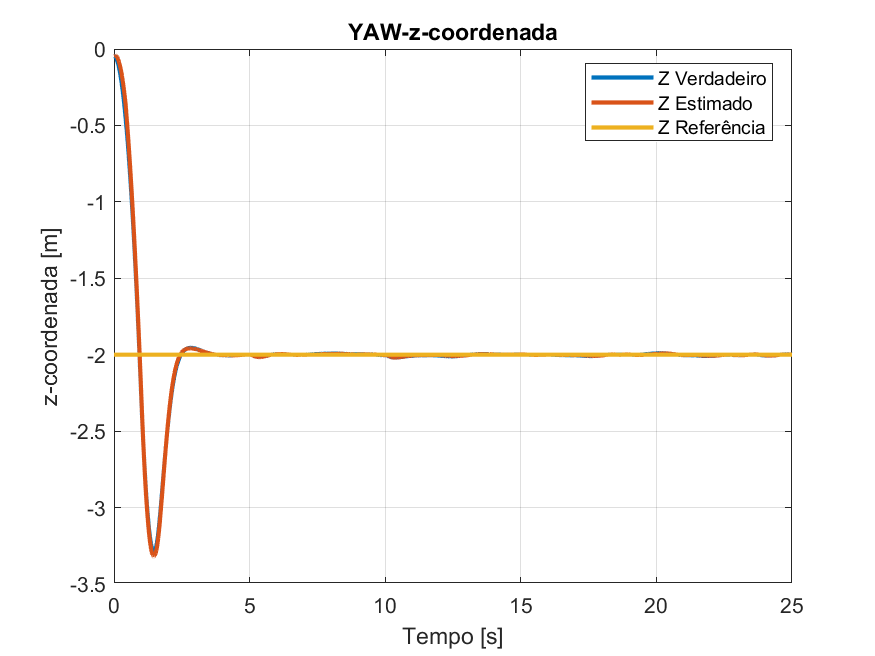
\includegraphics[width=0.8\textwidth]{YAW-z-coordenada.png}
    \caption{Coordenada Z para o Cenário de Mudança de Yaw}
    \label{fig:YAW-z-coordenada}
\end{figure}

Na coordenada Z (Figura \ref{fig:YAW-z-coordenada}), observamos que o sistema mantém a altitude de forma estável, mesmo com a variação de yaw. O controlador de altitude parece ser robusto o suficiente para não ser afetado pelas mudanças no yaw.

\begin{figure}[H]
    \centering
    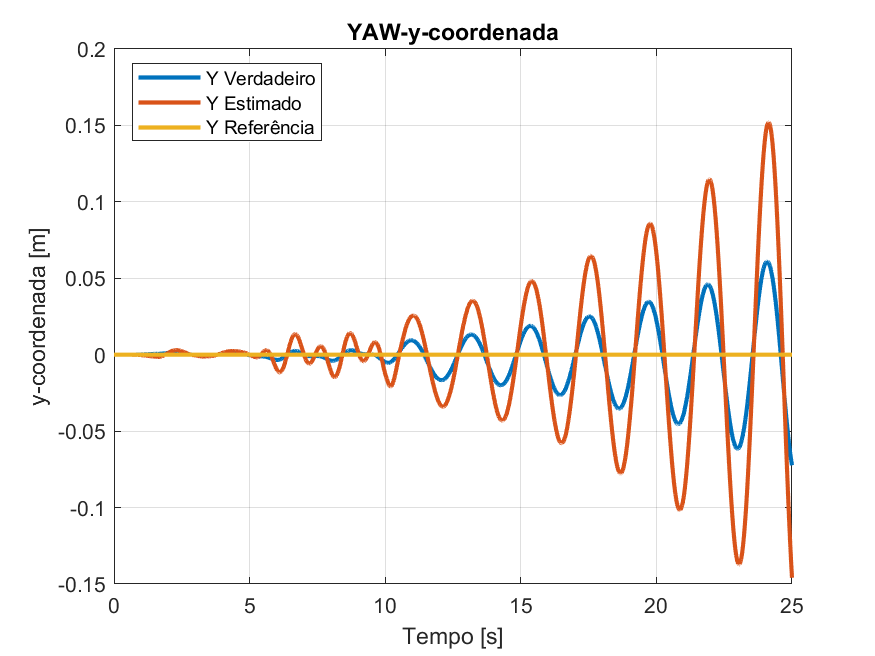
\includegraphics[width=0.8\textwidth]{YAW-y-coordenada.png}
    \caption{Coordenada Y para o Cenário de Mudança de Yaw}
    \label{fig:YAW-y-coordenada}
\end{figure}

A coordenada Y (Figura \ref{fig:YAW-y-coordenada}) apresenta um comportamento oscilatório leve, porém, devido à ação de yaw, o quadricóptero sofre pequenas variações de posição lateral. As oscilações são mínimas e não comprometem o controle de posição.

\begin{figure}[H]
    \centering
    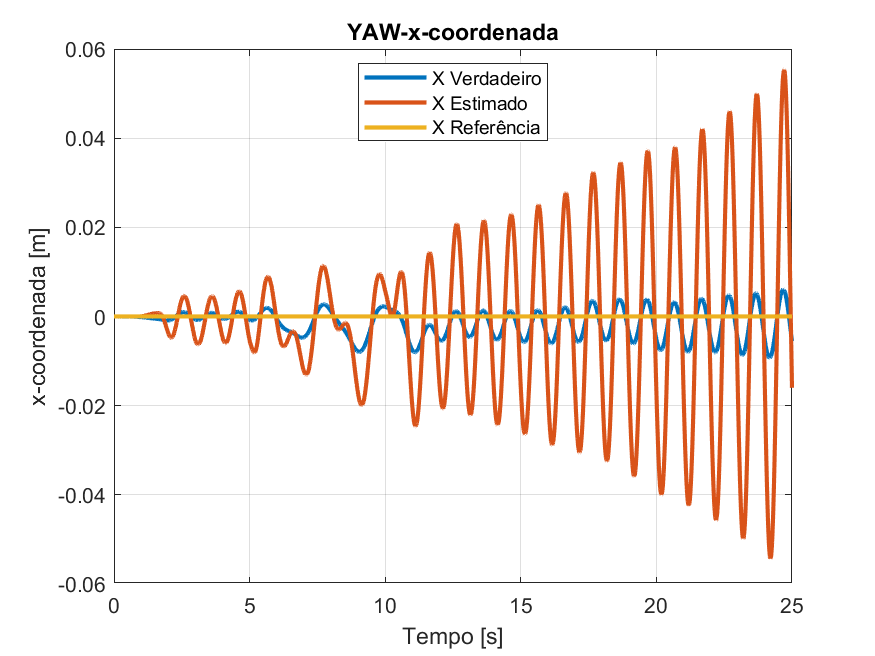
\includegraphics[width=0.8\textwidth]{YAW-x-coordenada.png}
    \caption{Coordenada X para o Cenário de Mudança de Yaw}
    \label{fig:YAW-x-coordenada}
\end{figure}

Na coordenada X (Figura \ref{fig:YAW-x-coordenada}), é possível observar um comportamento oscilatório similar ao observado em Y. O controlador mantém a estabilidade geral, mas há uma pequena resposta oscilatória induzida pela mudança de yaw.

%\textbf{Conclusão:} A resposta do quadricóptero no cenário de yaw é adequada e apresenta uma boa estabilidade. Embora pequenas oscilações apareçam nos eixos X, Y e nas atitudes de arfagem e rolagem, o controlador de yaw responde de maneira rápida e eficiente à mudança de referência. As oscilações são mínimas e poderiam ser ajustadas com um tuning fino, mas o desempenho geral é satisfatório para o cenário de mudança de yaw.



%---------------------------------------------------------------------
% INDICE REMISSIVO
%---------------------------------------------------------------------
\phantompart
\printindex
%---------------------------------------------------------------------
